\documentclass{standalone}

\usepackage{tikz}
\usetikzlibrary{decorations.markings}
\begin{document}



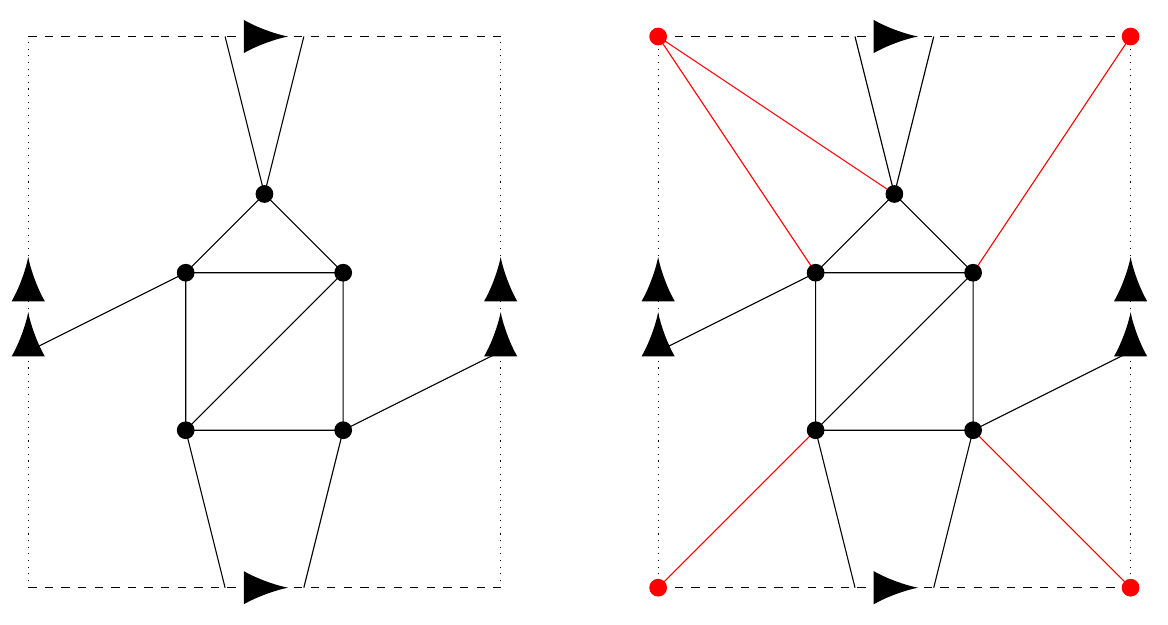
\begin{tikzpicture}

\draw[dashed,  
        decoration={markings, mark=at position 0.55 with {\arrow[scale=4]{latex}}},     postaction={decorate}
        ] (0,0)--(6,0);
\draw[dashed,        decoration={markings, mark=at position 0.55 with {\arrow[scale=4]{latex}}},     postaction={decorate}] (0,7)--(6,7);
\draw[dotted,        decoration={markings, mark=at position 0.5 with {\arrow[scale=4]{latex}}, mark=at position 0.6 with {\arrow[scale=4]{latex}}},    postaction={decorate}] (0,0)--(0,7);
\draw[dotted,        decoration={markings, mark=at position 0.5 with {\arrow[scale=4]{latex}}, mark=at position 0.6 with {\arrow[scale=4]{latex}}},     postaction={decorate}] (6,0)--(6,7);

\filldraw (2,2) circle(3pt);
\filldraw (2,4) circle(3pt);
\filldraw (4,2) circle(3pt);
\filldraw (4,4) circle(3pt);
\filldraw (3,5) circle(3pt);

\draw (2,2)--(2,4)--(4,4)--(4,2)--(2,2)--(4,4);
\draw (2,2)--(2.5,0);
\draw (3.5,0)--(4,2);
\draw (2.5,7)--(3,5)--(3.5,7);
\draw (2,4)--(3,5)--(4,4);
\draw (4,2)--(6,3);
\draw (0,3)--(2,4);


\begin{scope}[xshift=8cm]
\draw[dashed,  
        decoration={markings, mark=at position 0.55 with {\arrow[scale=4]{latex}}},     postaction={decorate}
        ] (0,0)--(6,0);
\draw[dashed,        decoration={markings, mark=at position 0.55 with {\arrow[scale=4]{latex}}},     postaction={decorate}] (0,7)--(6,7);
\draw[dotted,        decoration={markings, mark=at position 0.5 with {\arrow[scale=4]{latex}}, mark=at position 0.6 with {\arrow[scale=4]{latex}}},    postaction={decorate}] (0,0)--(0,7);
\draw[dotted,        decoration={markings, mark=at position 0.5 with {\arrow[scale=4]{latex}}, mark=at position 0.6 with {\arrow[scale=4]{latex}}},     postaction={decorate}] (6,0)--(6,7);

\begin{scope}[red]
\filldraw (0,0) circle (3pt);
\filldraw (6,0) circle (3pt);
\filldraw (6,7) circle (3pt);
\filldraw (0,7) circle (3pt);
\draw (0,0)--(2,2);
\draw (6,0)--(4,2);
\draw (6,7)--(4,4);
\draw (2,4)--(0,7)--(3,5);
\end{scope}


\filldraw (2,2) circle(3pt);
\filldraw (2,4) circle(3pt);
\filldraw (4,2) circle(3pt);
\filldraw (4,4) circle(3pt);
\filldraw (3,5) circle(3pt);

\draw (2,2)--(2,4)--(4,4)--(4,2)--(2,2)--(4,4);
\draw (2,2)--(2.5,0);
\draw (3.5,0)--(4,2);
\draw (2.5,7)--(3,5)--(3.5,7);
\draw (2,4)--(3,5)--(4,4);
\draw (4,2)--(6,3);
\draw (0,3)--(2,4);




\end{scope}
\end{tikzpicture} 


\end{document}
